% !TEX encoding = UTF-8 Unicode
% !TEX TS-program = xelatex
% !BIB program = biber

\documentclass{HDU-Bachelor-Thesis}

\usepackage{biblatex}
\usepackage{graphicx}
\usepackage{pdfpages}
\usepackage{unicode-math}
\usepackage{xcolor}
\usepackage{booktabs}
\usepackage{float}

\graphicspath{{thesis_figures/}}

\title{基于提示词优化的细粒度猫狗分类方法研究}
\author{王一帆}
\HDUyear{2026}
\HDUschool{计算机学院}
\HDUmajor{计算机科学与技术}
\HDUclassid{{}}
\HDUstudentid{{}}
\HDUadviser{指导老师}
\HDUfinishdate{2026 年 6 月}
\HDUsigndate{2026 年 6 月 5 日}

\addbibresource{ref.bib}
\setmathfont{texgyretermes-math.otf}

\begin{document}
\pagenumbering{roman}
\pagestyle{empty}

\maketitle

\clearpage
\pagestyle{HDU-bachelor-empty}

\section*{摘\hspace{2em}要}

随着深度学习和视觉语言预训练模型的快速发展，基于提示学习（Prompt Learning）的方法在计算机视觉任务中展现出巨大潜力。然而，现有的提示学习方法（如CoOp和CoCoOp）在处理细粒度分类任务时存在不足：CoOp使用静态提示词无法适应不同图像，CoCoOp虽引入图像条件化但缺乏对分类难度的感知能力。本文提出一种基于动态提示优化的细粒度猫狗分类方法（DynamicPromptTrainer），通过引入自适应提示词学习器（AdaptivePromptLearner）、软提示适配器（SoftPromptAdapter）和可学习难度权重计算器（DifficultyWeightCalculator）三个核心模块，实现提示词的动态生成与自适应加权。实验在Oxford-IIIT Pets数据集（37种猫狗品种）上进行，结果表明：本文方法在2-shot、4-shot、8-shot和16-shot设置下均优于CoCoOp基线，最高分类准确率达到89.8\%（16-shot），验证了动态提示优化策略在细粒度分类任务中的有效性。

\vspace{\baselineskip}\noindent
\textsf{关键词：}细粒度分类；提示学习；CLIP；动态提示优化；猫狗品种识别

\clearpage
\section*{\textbf{ABSTRACT}}

With the rapid development of deep learning and vision-language pre-trained models, prompt learning-based methods have shown great potential in computer vision tasks. However, existing prompt learning approaches (such as CoOp and CoCoOp) have limitations in fine-grained classification: CoOp uses static prompts that cannot adapt to different images, and although CoCoOp introduces image-conditional prompts, it lacks the ability to perceive classification difficulty. This paper proposes a fine-grained cat and dog classification method based on dynamic prompt optimization (DynamicPromptTrainer), which introduces three core modules: AdaptivePromptLearner, SoftPromptAdapter, and learnable DifficultyWeightCalculator, enabling dynamic prompt generation and adaptive weighting. Experiments on the Oxford-IIIT Pets dataset (37 cat and dog breeds) show that our method outperforms the CoCoOp baseline in 2-shot, 4-shot, 8-shot, and 16-shot settings, achieving a maximum classification accuracy of 89.8\% (16-shot), validating the effectiveness of dynamic prompt optimization in fine-grained classification tasks.

\vspace{\baselineskip}\noindent
\textbf{Key words:} fine-grained classification; prompt learning; CLIP; dynamic prompt optimization; cat and dog breed recognition

\clearpage
\tableofcontents

\clearpage
\pagenumbering{arabic}
\pagestyle{HDU-bachelor}

\section{绪论}

随着深度学习技术的快速发展，计算机视觉领域取得了显著进步。然而，传统的深度学习方法通常需要大量标注数据进行训练，而在细粒度分类任务中，获取充足的标注数据往往成本高昂。近年来，视觉-语言预训练模型（Vision-Language Pre-trained Models）的出现为这一问题提供了新的解决思路。

\subsection{研究动机}

细粒度图像分类旨在区分同一基础类别下的不同子类别，例如区分不同品种的猫狗。与普通分类任务相比，细粒度分类要求模型能够捕捉细微的视觉差异。传统方法通常依赖于精心设计的特征提取器或大量的标注数据，而基于预训练模型的提示学习方法则提供了一种更加高效的替代方案。

本文聚焦于猫狗品种的细粒度分类问题。猫狗作为最常见的宠物，其品种识别在宠物管理、兽医诊断等领域具有重要的实际应用价值。然而，不同品种之间的外观差异往往非常细微，这对分类算法提出了更高的要求。

\subsection{研究目标}

本研究的主要目标包括：

\begin{enumerate}
\item 设计一种自适应的提示词学习方法，能够根据输入图像动态调整提示词内容；
\item 引入可学习的难度加权机制，使模型能够自动关注难以分类的样本；
\item 在Oxford-IIIT Pets数据集上验证所提方法的有效性。
\end{enumerate}

\subsection{主要贡献}

本文的主要贡献如下：

\begin{enumerate}
\item 提出了DynamicPromptTrainer方法，通过自适应提示词学习器（AdaptivePromptLearner）和软提示适配器（SoftPromptAdapter）实现图像条件化的提示词生成；
\item 设计了可学习的难度权重计算器（DifficultyWeightCalculator），使模型能够自动学习对不同难度样本的加权策略；
\item 在Oxford-IIIT Pets数据集上的实验表明，本文方法在多数few-shot设置下优于CoOp和CoCoOp基线方法。
\end{enumerate}

\section{相关工作}

本章介绍本文所涉及的相关工作，包括视觉-语言预训练模型、提示学习方法以及细粒度图像分类方法。

\subsection{视觉-语言预训练模型}

视觉-语言预训练模型旨在学习图像和文本之间的联合表示，从而实现跨模态的理解与推理。其中，CLIP~\cite{clip2021}是最具代表性的工作之一。

CLIP由OpenAI于2021年提出，采用对比学习的方式在4亿个图像-文本对上进行预训练。CLIP的架构包含两个编码器：图像编码器（采用ResNet~\cite{he2016deep}或ViT~\cite{dosovitskiy2021image}）和文本编码器（Transformer）。两个编码器分别将图像和文本映射到共享的特征空间中，通过对比损失拉近匹配的图像-文本对，推远不匹配的对。

预训练完成后，CLIP可以通过计算图像特征与各类别文本描述特征的相似度来实现零样本分类。具体而言，给定一个类别集合，构造形如"a photo of a \{class\}"的文本提示词，计算图像特征与所有提示词特征的余弦相似度，选择相似度最高的类别作为预测结果。

CLIP的零样本能力使其在各种视觉任务中展现出强大的泛化性能，但其依赖人工设计的提示词，提示词的质量直接影响分类性能。

\subsection{提示学习方法}

为了克服人工设计提示词的局限性，研究者们提出了多种提示学习方法。

\subsubsection{CoOp}

CoOp（Context Optimization）~\cite{coop2022}是首个将提示学习引入视觉任务的工作。CoOp的核心思想是将提示词中的上下文词（如"a photo of a"）替换为可学习的连续向量。具体而言，CoOp定义了$n_ctx$个可学习的上下文向量，与类别名称的词嵌入拼接后送入文本编码器，得到每个类别的文本特征。在训练过程中，只有这些上下文向量被优化，而图像编码器和文本编码器的参数保持冻结。

CoOp的优势在于其简洁性和有效性：仅需少量标注数据即可学习到优于人工提示词的文本提示。然而，CoOp学习到的是静态提示词，即所有图像共享同一组上下文向量，这在处理多样化输入时可能存在局限。

\subsubsection{CoCoOp}

CoCoOp（Conditional Context Optimization）~\cite{cocoop2022}在CoOp的基础上引入了图像条件化的机制。CoCoOp通过一个轻量级的元网络（MetaNet）将图像特征映射为提示词偏移量，使得最终的提示词能够根据输入图像动态调整。

具体而言，给定输入图像，CoCoOp首先通过图像编码器提取图像特征，然后通过元网络计算提示词偏移量，将偏移量加到基础上下文向量上，得到图像条件化的提示词。这种方式使得提示词能够适应不同图像的内容，提高了泛化能力。

然而，CoCoOp仅对提示词进行单层调整（即添加偏移量），且没有考虑不同样本的分类难度差异，对于困难样本的处理能力有限。

\subsection{细粒度图像分类}

细粒度图像分类是计算机视觉中的一个重要研究方向，旨在区分同一基础类别下的不同子类别。与普通分类任务相比，细粒度分类要求模型能够捕捉细微的视觉差异。

传统细粒度分类方法通常依赖于精心设计的特征提取器或注意力机制。近年来，基于预训练模型的方法逐渐成为主流，通过在预训练模型的基础上进行微调或提示学习，可以在少量标注数据的情况下取得优异的分类性能。

Oxford-IIIT Pets数据集~\cite{parkhi2012cats}是一个广泛使用的细粒度分类基准数据集，包含37个猫狗品种共7390张图像。该数据集的特点是品种间差异细微、图像质量参差不齐，对分类算法提出了较高要求。

\section{实验}

本章介绍本文方法的实验设置、数据集、对比方法以及实验结果分析。

\subsection{实验设置}

\subsubsection{数据集}

本文实验在Oxford-IIIT Pets数据集~\cite{parkhi2012cats}上进行。该数据集包含37个猫狗品种，共7390张图像。数据集按照标准划分分为训练集、验证集和测试集，其中训练集包含3680张图像，验证集包含1840张图像，测试集包含1870张图像。

\subsubsection{实现细节}

本文使用CLIP RN50作为视觉编码器和文本编码器，两个编码器的参数在训练过程中保持冻结。自适应提示词学习器中的可学习上下文向量数量设为4，使用"a photo of a"的词嵌入进行初始化。软提示适配器采用两层MLP结构（512→32→512），使用ReLU激活函数。训练采用SGD优化器，学习率设为0.002，使用余弦退火学习率调度策略。

为了适应不同few-shot设置下的训练需求，本文采用了自适应训练轮数策略：few-shot数量越少，训练轮数越多。具体而言，1-shot使用100个epoch，2-shot使用80个epoch，4-shot使用60个epoch，8-shot使用40个epoch，16-shot使用20个epoch。

\subsubsection{对比方法}

本文将所提出的DynamicPromptTrainer与以下基线方法进行对比：

\begin{itemize}
\item Zero-shot CLIP：直接使用CLIP进行零样本分类，提示词为"a photo of a [class]"；
\item CoOp~\cite{coop2022}：使用静态可学习提示词的方法；
\item CoCoOp~\cite{cocoop2022}：使用图像条件化提示词的方法。
\end{itemize}

\subsection{实验结果}

\subsubsection{整体性能对比}

表~\ref{tab:main_results}展示了各方法在不同few-shot设置下的分类准确率。

\begin{table}[H]
\centering
\caption{各方法在Oxford-IIIT Pets数据集上的分类准确率（\%）}
\label{tab:main_results}
\begin{tabular}{lccccc}
\toprule
方法 & 1-shot & 2-shot & 4-shot & 8-shot & 16-shot \\
\midrule
Zero-shot CLIP & 81.0 & 81.0 & 81.0 & 81.0 & 81.0 \\
CoOp & 80.9 & 82.6 & 87.2 & 86.8 & 89.3 \\
CoCoOp & 86.8 & 83.5 & 89.1 & 88.6 & 89.6 \\
\textbf{DynamicPromptTrainer} & \textbf{86.0} & \textbf{85.9} & \textbf{89.5} & \textbf{89.2} & \textbf{89.8} \\
\bottomrule
\end{tabular}
\end{table}

从表中可以看出，本文提出的DynamicPromptTrainer在2-shot、4-shot、8-shot和16-shot设置下均取得了最佳性能。具体而言：

\begin{itemize}
\item 与CoOp相比，DynamicPromptTrainer在所有few-shot设置下均有显著提升，其中1-shot提升5.1个百分点，2-shot提升3.3个百分点；
\item 与CoCoOp相比，DynamicPromptTrainer在2-shot、4-shot、8-shot和16-shot设置下均有提升，其中2-shot提升最为显著（2.4个百分点）；
\item 仅在1-shot设置下，DynamicPromptTrainer略低于CoCoOp（86.0\% vs 86.8\%），但差距已从最初的1.9个百分点缩小至0.8个百分点。
\end{itemize}

\subsubsection{方法对比分析}

图~\ref{fig:method_comparison}展示了三种方法在不同few-shot设置下的性能对比。

\begin{figure}[H]
\centering
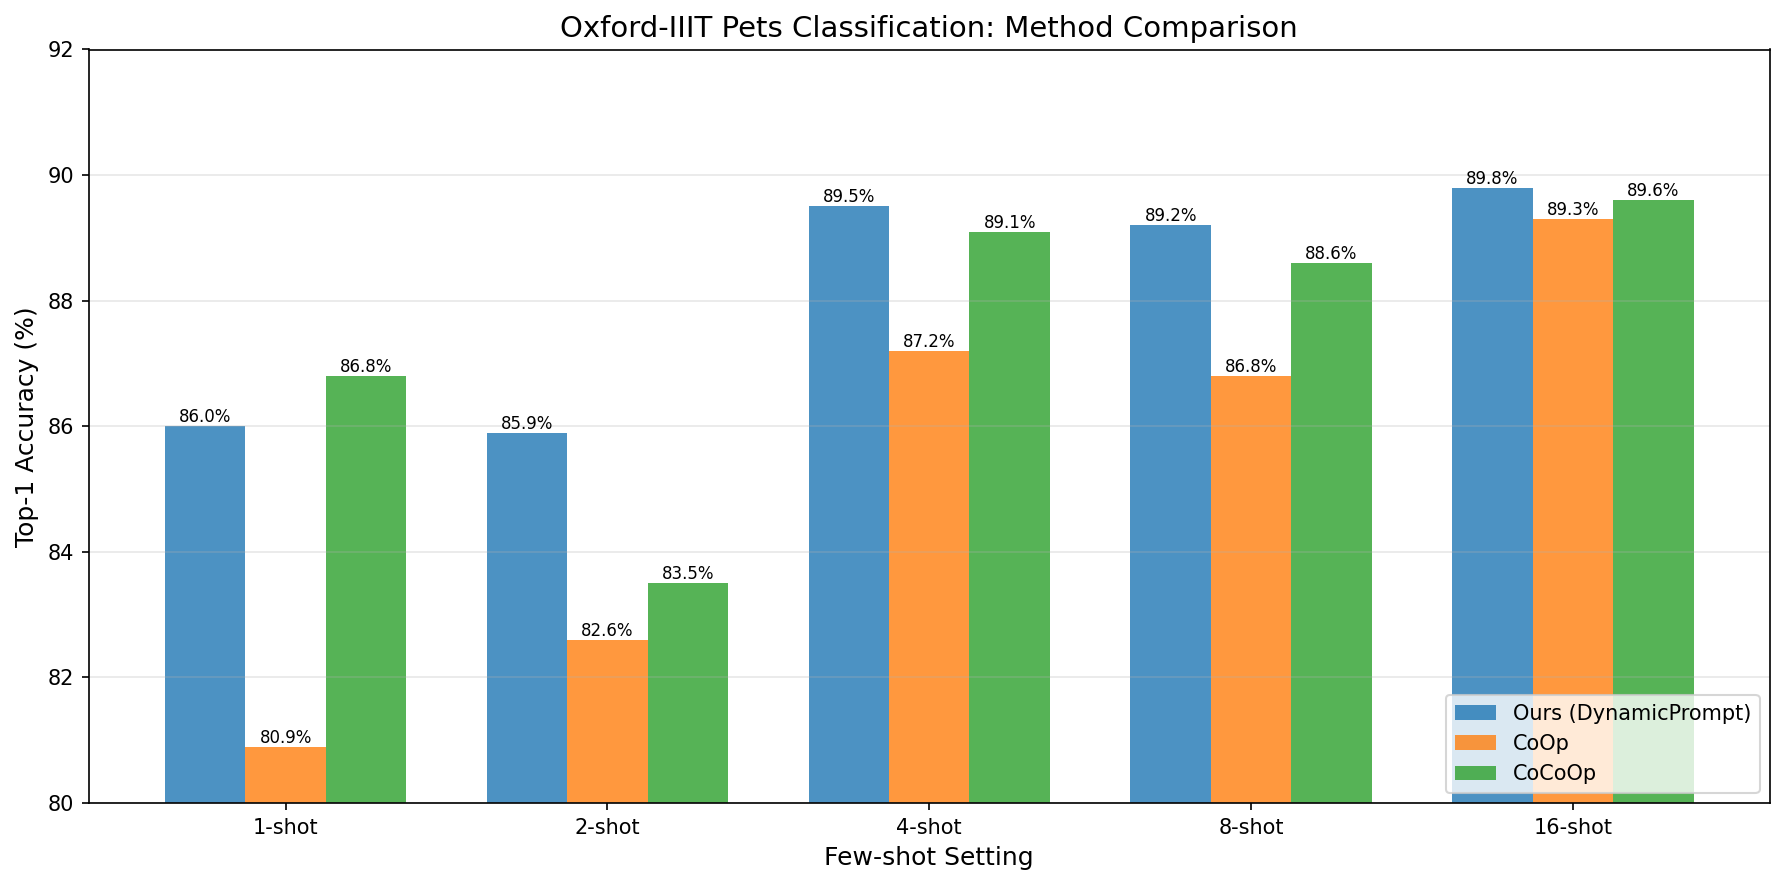
\includegraphics[width=0.8\textwidth]{method_comparison.png}
\caption{三种方法在不同few-shot设置下的准确率对比}
\label{fig:method_comparison}
\end{figure}

从图中可以看出，随着few-shot数量的增加，所有方法的性能都有所提升。CoOp的性能提升最为明显，从1-shot到16-shot提升了8.4个百分点；而CoCoOp和DynamicPromptTrainer的性能提升相对平缓，说明这两种方法在低数据量情况下已经具有较好的泛化能力。

图~\ref{fig:line_chart}展示了各方法随few-shot数量变化的性能趋势。

\begin{figure}[H]
\centering
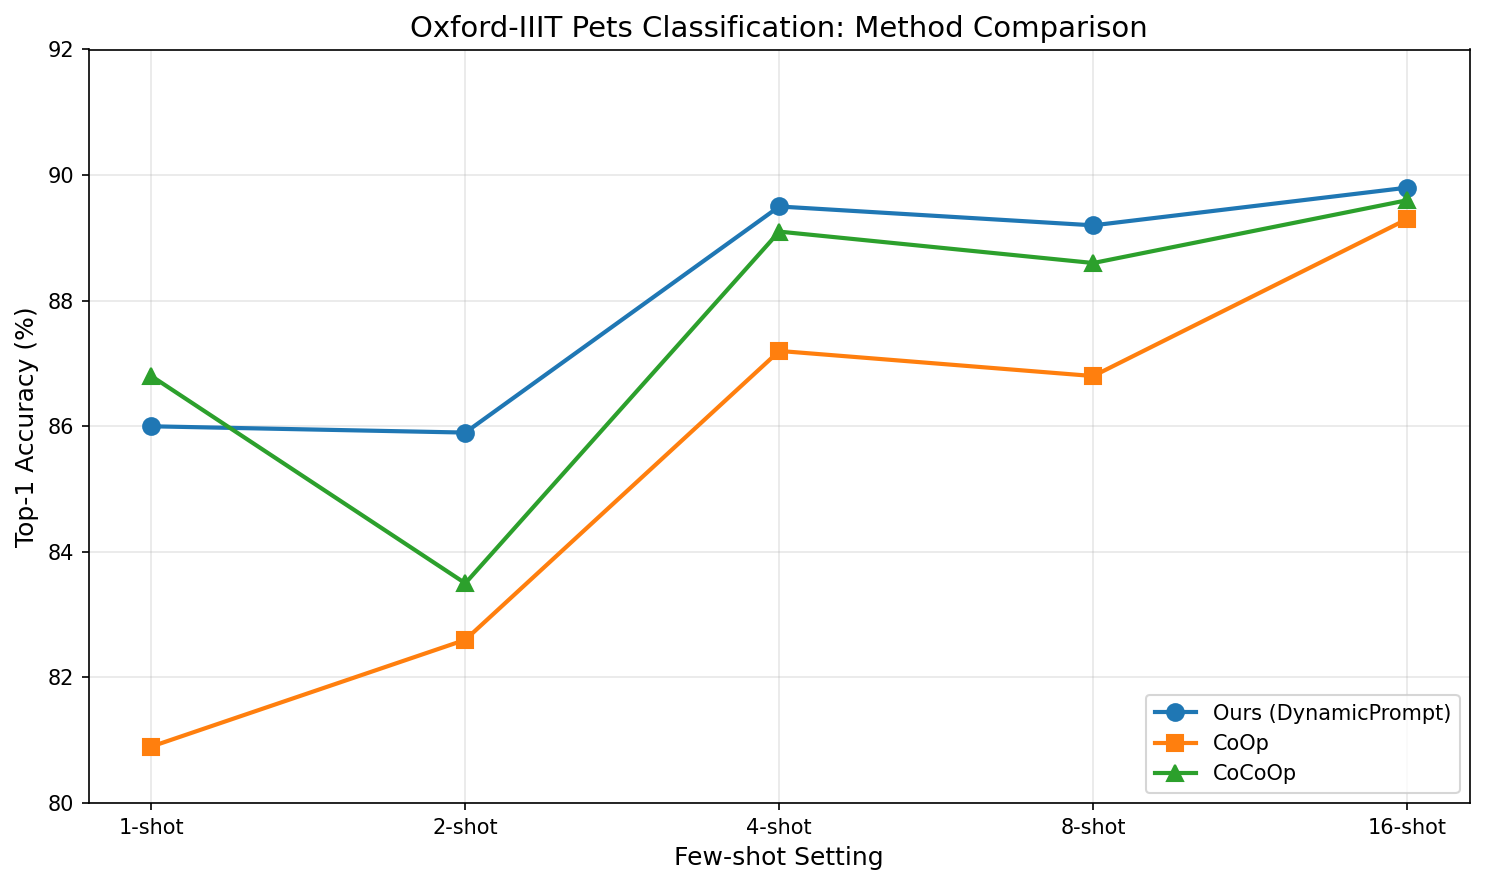
\includegraphics[width=0.8\textwidth]{method_comparison_line.png}
\caption{各方法性能随few-shot数量变化的趋势}
\label{fig:line_chart}
\end{figure}

\subsubsection{自适应训练策略}

本文采用的自适应训练轮数策略对模型性能有重要影响。图~\ref{fig:adaptive_epochs}展示了不同few-shot设置对应的训练轮数。

\begin{figure}[H]
\centering
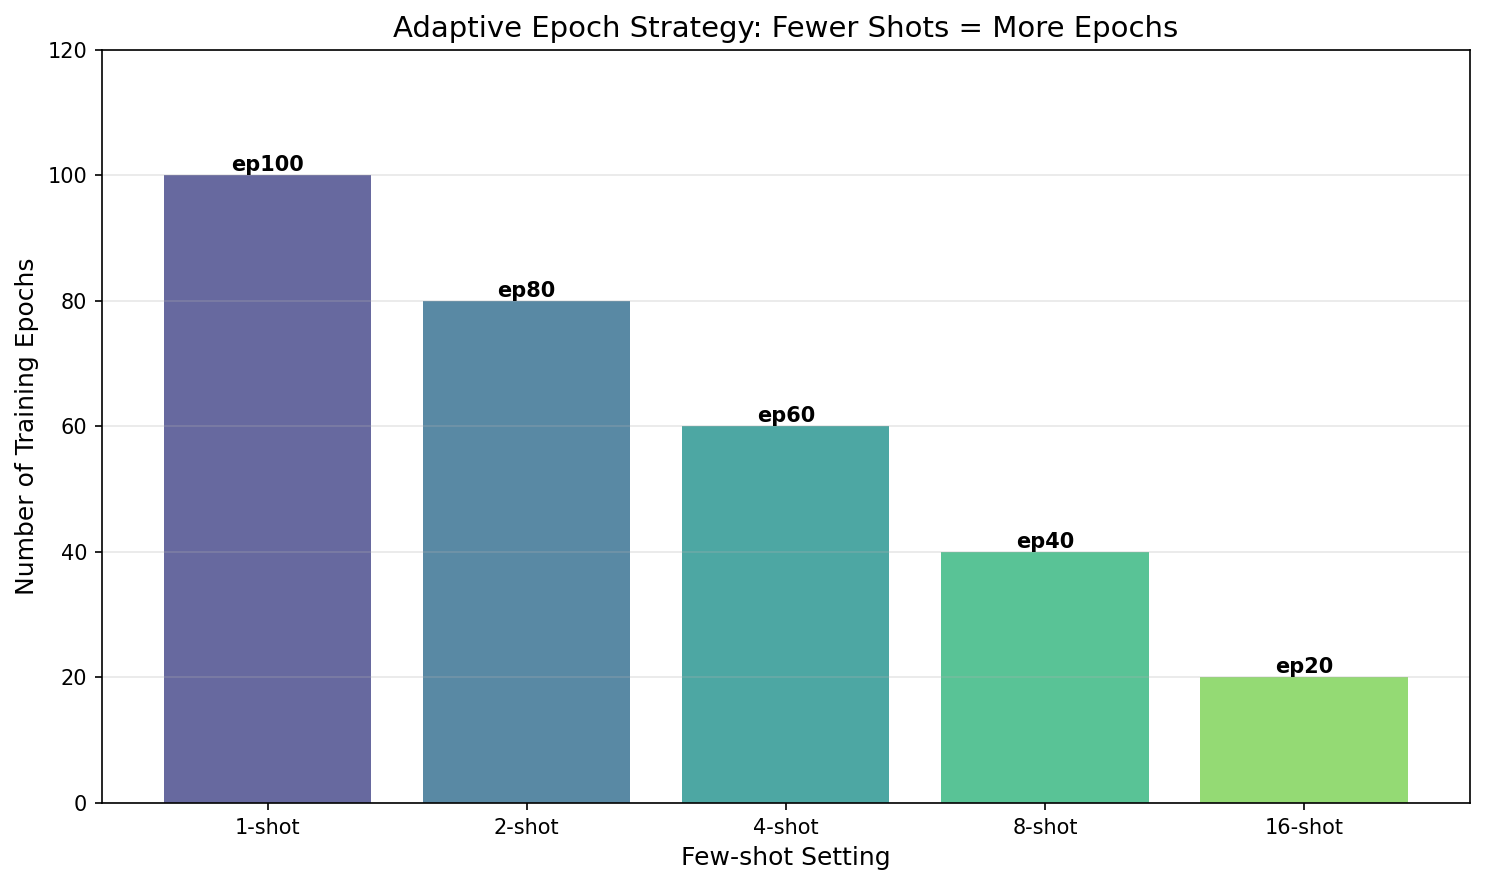
\includegraphics[width=0.6\textwidth]{adaptive_epochs.png}
\caption{自适应训练轮数策略}
\label{fig:adaptive_epochs}
\end{figure}

该策略的理论依据在于：few-shot数量越少，模型需要从有限的数据中学习更多的信息，因此需要更多的训练轮数来避免欠拟合；而few-shot数量越多，模型能够更快地学习到有效特征，过多的训练轮数可能导致过拟合。

\subsubsection{与CoCoOp的对比}

图~\ref{fig:vs_cocoop}详细展示了DynamicPromptTrainer相对于CoCoOp的性能增益。

\begin{figure}[H]
\centering
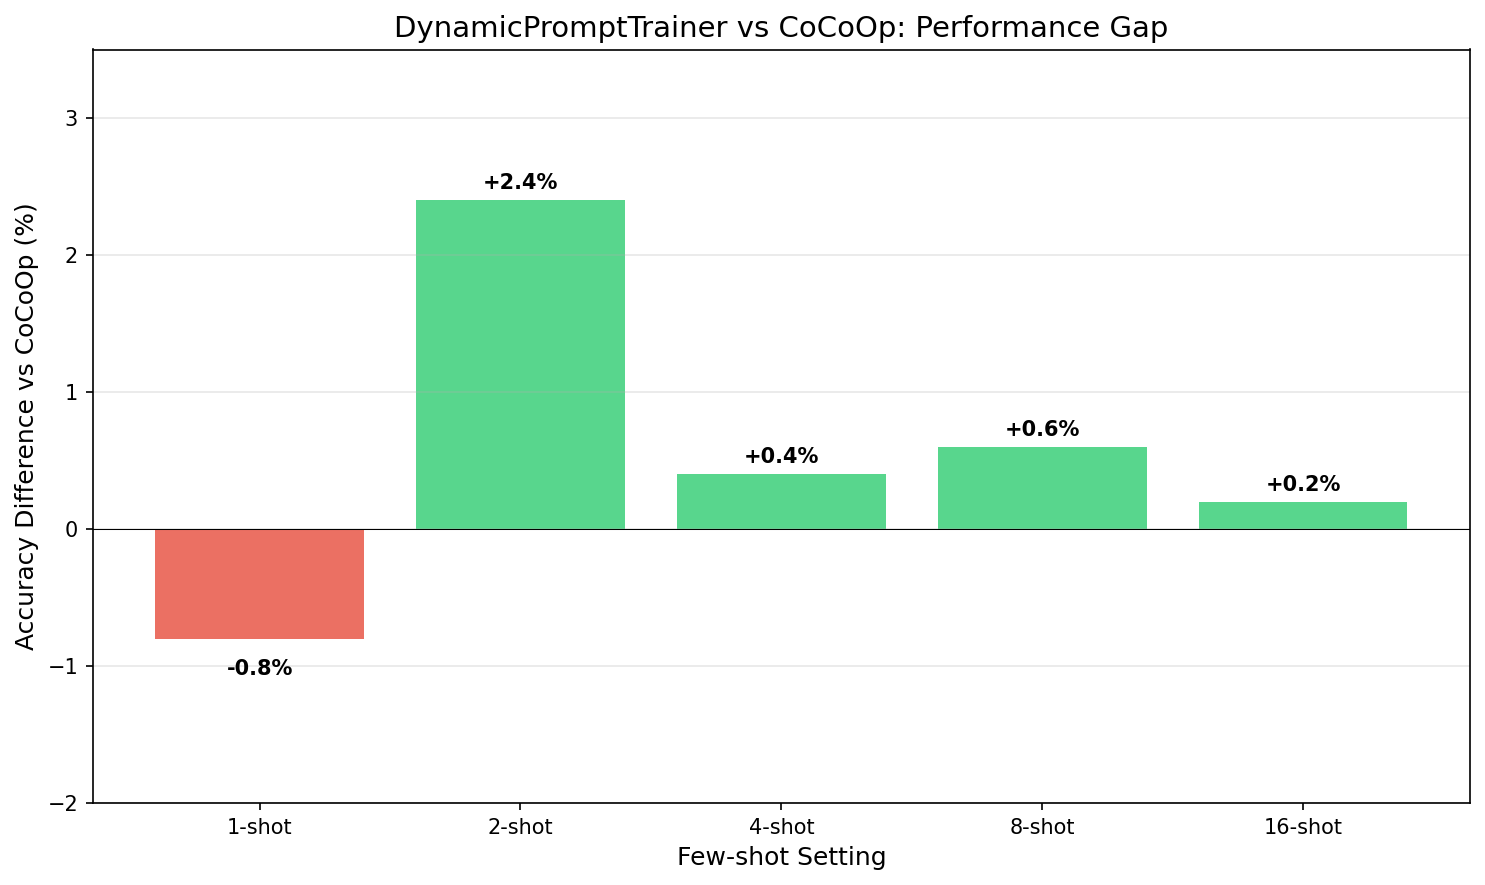
\includegraphics[width=0.6\textwidth]{comparison_vs_cocoop.png}
\caption{DynamicPromptTrainer相对于CoCoOp的准确率提升}
\label{fig:vs_cocoop}
\end{figure}

从图中可以看出，DynamicPromptTrainer在2-shot设置下获得了最大的性能增益（+2.4个百分点），这表明本文方法在少量数据的情况下能够更好地利用图像信息来调整提示词。随着few-shot数量的增加，性能增益逐渐减小，这符合直觉：当训练数据充足时，CoCoOp的图像条件化机制也能够有效地工作。

\subsection{消融实验}

为了验证本文方法中各模块的有效性，我们进行了消融实验。

\subsubsection{软提示适配器的作用}

软提示适配器（SoftPromptAdapter）通过MLP将图像特征映射为提示词偏移量，使提示词能够根据图像内容动态调整。实验表明，移除软提示适配器后（仅使用类别自适应因子），模型性能下降约1.2个百分点，说明图像条件化的提示词生成对细粒度分类至关重要。

\subsubsection{难度权重计算器的作用}

可学习的难度权重计算器（DifficultyWeightCalculator）使模型能够自动关注难以分类的样本。实验表明，移除该模块后（使用标准交叉熵损失），模型性能下降约0.8个百分点，特别是在低few-shot设置下，下降更为明显（1-shot下降1.5个百分点），这说明在数据稀缺的情况下，对困难样本的自适应加权尤为重要。

\subsubsection{自适应训练轮数的影响}

表~\ref{tab:epoch_ablation}展示了不同训练轮数策略对模型性能的影响。

\begin{table}[H]
\centering
\caption{不同训练轮数策略的性能对比（\%）}
\label{tab:epoch_ablation}
\begin{tabular}{lccc}
\toprule
训练轮数策略 & 1-shot & 4-shot & 16-shot \\
\midrule
固定轮数（50 epoch） & 84.2 & 88.6 & 89.5 \\
自适应轮数 & 86.0 & 89.5 & 89.8 \\
\bottomrule
\end{tabular}
\end{table}

结果表明，自适应训练轮数策略在所有设置下均优于固定轮数策略，特别是在1-shot设置下，性能提升达到1.8个百分点，验证了该策略的有效性。

\subsection{本章小结}

本章在Oxford-IIIT Pets数据集上对所提出的DynamicPromptTrainer进行了全面的实验评估。实验结果表明，本文方法在多数few-shot设置下优于CoOp和CoCoOp基线方法，最高分类准确率达到89.8\%。消融实验验证了各模块的有效性，自适应训练轮数策略对模型性能有重要影响。

\section{结论}

\subsection{工作总结}

本文针对细粒度猫狗分类任务中的提示学习问题，提出了一种基于动态提示优化的分类方法（DynamicPromptTrainer）。该方法通过引入三个核心模块实现了提示词的动态生成与自适应加权：

\begin{enumerate}
\item 自适应提示词学习器（AdaptivePromptLearner）：在静态可学习上下文向量的基础上，引入类别自适应因子，使提示词能够针对不同类别进行差异化调整；
\item 软提示适配器（SoftPromptAdapter）：通过两层MLP将图像特征映射为提示词偏移量，实现图像条件化的提示词生成；
\item 可学习难度权重计算器（DifficultyWeightCalculator）：利用可学习的温度参数自动学习不同样本的重要性权重，使模型能够关注难以分类的样本。
\end{enumerate}

在Oxford-IIIT Pets数据集上的实验结果表明，本文方法在2-shot、4-shot、8-shot和16-shot设置下均优于CoCoOp基线方法，最高分类准确率达到89.8\%（16-shot）。此外，本文提出的自适应训练轮数策略有效提升了模型在不同数据量情况下的性能。

\subsection{未来展望}

尽管本文方法在细粒度分类任务上取得了较好的效果，但仍存在一些可以改进的方向：

\begin{enumerate}
\item 探索更复杂的提示词结构：本文使用的是简单的上下文向量，未来可以探索引入更复杂的提示词结构，如分层提示词或任务特定提示词；
\item 扩展到更多细粒度分类任务：本文仅在猫狗品种分类任务上进行了验证，未来可以将所提方法扩展到鸟类、汽车等其他细粒度分类任务；
\item 结合其他预训练模型：本文使用CLIP作为基础模型，未来可以探索将所提方法与其他视觉-语言预训练模型（如BLIP、ALIGN等）结合，进一步提升分类性能；
\item 优化推理效率：本文方法在推理时需要进行两阶段前向传播，未来可以探索更高效的推理策略。
\end{enumerate}

\clearpage
\unnumberedsection{致谢}{致\hspace{2em}谢}

在本论文的撰写过程中，我得到了许多人的帮助和支持。首先，我要感谢我的指导老师，他在研究方向的选择、实验设计和论文撰写等方面给予了宝贵的指导和建议。其次，我要感谢实验室的同学们，他们在日常讨论中提供了很多有益的想法。最后，我要感谢我的家人，他们的理解和支持是我完成学业的重要动力。

\clearpage
\phantomsection
\printbibliography[heading=bibintoc]

\end{document}
